\documentclass[12pt]{article}

\usepackage{tikz}
\usepackage[ruled, vlined]{algorithm2e}
\usepackage{pst-node,pst-plot}
\usepackage{amsmath}
\usepackage{float}

\newcommand{\BigO}[1]{\ensuremath{\operatorname{\mathcal{O}}\bigl(#1\bigr)}}

\begin{document}
\title{Homework 14}
\author{Robbie McKinstry, Jack McQuown, Cyrus Ramavarapu}
\renewcommand{\today}{3 October 2016}
\renewcommand{\baselinestretch}{1.5}
\maketitle

\section*{Dynamic Programming}
\subsection*{Problem 24:}
\subsection*{Problem 27:}

\section*{Reductions}
\subsection*{Problem 2:}
A relationship between inverting a matrix and multiplying arbitrary
square matrices can be developed to show that if there exists a
\BigO{n^k} for $k\geq2$ for matrix inversion ($MI$), a \BigO{n^k} algorithm
for matrix multiplication ($MM$) can also be found.  Essentially, this
means the following.
\[
Matrix\ Multiplication\leq_{p} Matrix\ Inversion  
\]
This reduction means that there exists an incomplete algorithm for
MM that at some point calls an algorithm for MI\@.  Prior to making the
call to MI, MM must transform its input, arbitrary matrices $A$ and $B$,
into an appropriate form for MI, a nonsignular matrix.  Additionally,
the output of MI will have to be transformed into the output of MM,
which is the product $AB$. Since, the  algorithm for MI operates in
\BigO{n^k} time for $k\geq2$, the two transformations must occur in
at most \BigO{n^k} time, otherwise the transformation will become
the rate limiting step. Pictorially this can be represented in the
following arrow diagram.
\begin{center}
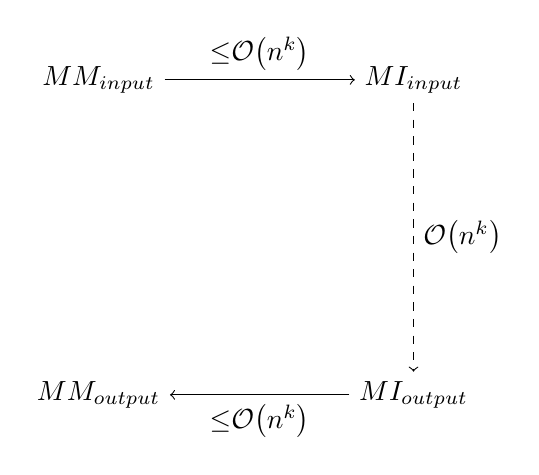
\begin{tikzpicture}[node distance=4cm, auto]
    \node (S) {$MM_{input}$};
    \node (F) [below of=S] {$MM_{output}$};
    \node (Mo) [right of=F] {$MI_{output}$};
    \node (Mi) [right of=S] {$MI_{input}$};
    \draw[->] (S) to node {$\leq$\BigO{n^k}} (Mi);
    \draw[->, dashed] (Mi) to node {\BigO{n^k}} (Mo); 
    \draw[->] (Mo) to node {$\leq$\BigO{n^k}} (F);
\end{tikzpicture}
\end{center}

Using the above diagram as a guideline, the following transformation
can be considered.  Given two arbitrary matrices $A$ and $B$ as input
to MM, a new matrix $Z$ can be created as follows.
\[
Z =
    \begin{pmatrix}
    I & A & 0 \\
    0 & I & B \\
    0 & 0 & I 
    \end{pmatrix}
\]
To show that $Z$ constitutes appropriate input for $MI$ is a straight
forward process using the Laplace expansion for determinants to show
that $\det(Z)$ is $1$ and hence nonzero and independent of $A$ and $B$.\\\\
Although the details of the \BigO{n^k} algorithm for matrix inversion
are unknown, the inverse can be found through a slower procedure and 
used as output of $MI$.\footnote{Matrix inverse are unique.  This can
be easily showed by assuming two matrices $A$ and $B$ have the same inverse
$C$.  Therefore the following holds.
\[
A = AI = A(CB) = (AC)B = IB = B
\]
}
Consequently, $Z^{-1}$ can be found by performing Gaussian elimination
on $[Z|I]$ and converting it into $[I|Z^{-1}]$.  This process yields the
following value for $Z^{-1}$.
\[
Z^{-1} =
    \begin{pmatrix}
    I & -A & AB \\
    0 & I & -B \\
    0 & 0 & I 
    \end{pmatrix}
\]
Since this is the output of $MI$, it must be transformed into the output
of $MM$ using a process that is maximally \BigO{n^k} for $k\geq2$.  The
output of $MM$ is the product $AB$, which can be recovered by searching 
all the values in $Z^{-1}$.  This value can then be returned from $MM$.\\\\
This method of matrix multiplication had two transformations, creating
$Z$ and searching $Z^{-1}$, both of which take \BigO{n^2} time.  As a result
the entire process will be bounded by $MI$ and will therefore be at least
\BigO{n^2} due to the restriction placed on $k$.
\subsection*{Problem 4:}
A relationship between a varient of the minimum Steiner tree problem ($STP$) and 
sorting ($SRT$) can be developed to show that if the Steiner tree can be formed
in \BigO{n} time, a set of numbers can also be sorted in \BigO{n}.  Essentially,
this means that $SRT$ is reducible to $STP$.
\[
Sorting \leq_{p} Minimum\ Steiner\ Tree
\]
This reduction means that there exists an incomplete algorithm for $SRT$ 
that at some point calls the algorithm for $STP$.  However, since the 
the input for $SRT$ is a set of numbers, $\mathcal{N}$, and the input for 
$STP$ is a set of of points, $\mathcal{P}$, $SRT$ will have to transform its
input into an appropriate input for $STP$.  Similarily, the adjacency list
$STP$ outputs to represent the tree will have to transformed into the output
for $SRT$.  Both of these transformations must occur in at most \BigO{n} time,
otherwise they will become the rate limiting step in the sorting algorithm. This
relationship between the two algorithms can be represented pictorially as follows. 
\begin{center}
\begin{tikzpicture}[node distance=4cm, auto]
    \node (S) {$SRT_{input}$};
    \node (F) [below of=S] {$SRT_{output}$};
    \node (STPo) [right of=F] {$STP_{output}$};
    \node (STPi) [right of=S] {$STP_{input}$};
    \draw[->] (S) to node {$\leq$\BigO{n}} (Mi);
    \draw[->, dashed] (Mi) to node {\BigO{n}} (Mo); 
    \draw[->] (Mo) to node {$\leq$\BigO{n}} (F);
\end{tikzpicture}
\end{center}
One possible transform to apply on $\mathcal{N}$ so that it is acceptable input 
for $STP$ is to map every element in $\mathcal{N}$ onto the $x\ axis$.
\[
    \forall n\in\mathcal{N}:n\rightarrow(n,0)
\]
When the \BigO{n} algorithm for $STP$ operates on these points, it will only connect
adjacent points together because each point must be reachable from any other point
and roads may not cross.  As a result, if the set of points given to $STP$ is
$\{(0,0),(1,0),(2,0),(3,0)\}$ the following adjacency list will be produced.
\begin{center}
\begin{tabular}{c|c}
Point & Adjacents\\ \hline
(0,0) & (1,0)\\
(1,0) & (0,0) (2,0)\\
(2,0) & (1,0) (2,0)\\ 
(3,0) & (2,0)\\
\end{tabular} 
\end{center}
To transform the adjacency list output of $STP$ into a sorted list for $SRT$, the
smallest within the adjacency list must be found.  This can be done by going through 
the list of points and keeping track of the element with the smallest abscissa.  Once
this element is found, the adjacency list can be followed from this point only
considering points that have not already been seen.  With the exception of the 
end points, where $1$ point is adjacent, only $2$ points will have to be considered
at every point visited to determine which point is new.\\\\
The two transformations performed in this version of the $SRT$ algorithm both 
occur in \BigO{n} time because each process requires iterating through all the elements.
Mapping the $SRT$ input onto the real line requires a conversion of each element and 
finding the element with the minimum abscissa in the adjacency list is also a linear
search.  The last transformation requries looking at $2n$ items because each internal
point on the line will have two points adjacent.  Since each intermediate step only takes
\BigO{n} time, sorting will occur in \BigO{n} time. 
\end{document}
